\documentclass[a4,10pt, fleqn]{article}  %@@
%\usepackage[dvips]{epsfig}
\usepackage{amsmath,amssymb,comment}
\usepackage{graphicx,multicol}
\oddsidemargin -0.2in %-0.4in for smaller margins
\topmargin -1.25in %-1in (for above)
\textheight 10in %10.75in (for above)
\textwidth 6.75in %6.75in (for above)
\parindent=0pt
%\pagestyle{headings}%{headings}if you want page numbers top right

%***************************************************************************
%\pagestyle{myheadings}for header and pagenumber with \markright{\rm...{  }}
%e.g.  \markright{\rm{HG123\ Fourier}}
%use with \thispagestyle{empty} after begin document

%***************************************************************************
\newcommand{\ds}{\displaystyle}%display maths
\newcommand{\sst}{\scriptstyle}%very small maths
\newcommand{\sm}{\textstyle}%normal size maths
\newcommand{\bm}[1]{\mbox{\boldmath{$#1$}}}
\newcommand{\rom}[1]{\mbox{${\rm#1}$}}%roman in maths
\newcommand{\pa}{\partial}
\newcommand{\ep}{\varepsilon}
\newcommand{\na}{\bm\nabla}
\newcommand{\blR}{\rom{I\!R}}
\newcommand{\blI}{\rom{I\!I}}
\newcommand{\there}{$\dot{.\ .}$}
\renewcommand{\it}{\textit}
\renewcommand{\sc}{\textsc}
\renewcommand{\rm}{\textrm}
\newcommand{\ve}[1]{\mbox{$#1$}}
\newcommand{\veT}[1]{\mbox{$#1$}^{\operatorname{T}}}
\newcommand{\tr}{\mbox{Tr}}
\newcommand{\R}{\mathbb{R}}
\renewcommand{\d}{\mathrm{d}}
\newcommand{\norm}[1]{|\!| #1 |\!|}
\newcommand{\ip}[2]{<#1,#2>}
\newcommand{\dd}{\mbox{\,d}}


\def\be{\begin{equation}}
\def\ee{\end{equation}}
\def\ba{\begin{array}}
\def\ea{\begin{array}}
\newcommand{\bea}{\begin{eqnarray}}
\newcommand{\eea}{\end{eqnarray}}
\newcommand{\beas}{\begin{eqnarray*}}
\newcommand{\eeas}{\end{eqnarray*}}
\newcommand{\beg}{\begin{eqngroup}}
\newcommand{\eeg}{\end{eqngroup}}
\newcommand{\nno}{\nonumber}
\def \ptl{\partial}



%***************************************************************************
\begin{document}
\sffamily%@@
\thispagestyle{empty}
\begin{center}
University of Nottingham\\
School of Mathematical Sciences
\end{center}
%***************************************************************************
\large\textsc {MATH4063}\hfill\large\textsc {Scientific Computing and C++}%dont forget to
%change these
%\begin{comment}

\vspace*{2ex}
\hrule
\vskip0.25cm
\textbf{Suggested Submission Date: Monday 23rd November 2020, 2pm}
\hfill \textbf{Coursework 1}\\

\noindent
{\em Your results to the assessed coursework may be submitted using
this template. Please cut and paste the subsequent output into the correct parts
of this file and replace the placeholder \verb|solution.jpg| plots with your own. Once this
template has been completed, you must then create a pdf file for submission. Under Windows or Mac you can use Texmaker + a LaTeX compiler; from the Windows Virtual Desktop this may be accessed as follows:
\begin{verbatim}
Start > UoN Applications > (UoN) Texmaker 5
\end{verbatim}
 Open this file under {\tt File}; to build the pdf file, click the arrow next to {\tt Quick Build}; this will then generate the file Coursework1\_submission.pdf.\\

{\bf A single zip file containing your solution should be submitted} on Moodle. {\bf Note:}  All parameters and values should be set within your codes: do NOT use inputs such as those obtained with {\tt std::cin}.
}
%\end{comment}

Your code should be separated into a folder \verb|main|, with subfolders \verb|source| and \verb|include| as follows:

\vspace*{0.3cm}
{\bf File checklist:} \\
Coursework1\_submission.pdf
 \begin{multicols}{3}
\textbf{main:}
\begin{itemize}
\item Q1c.cpp
\item Q2b.cpp
\item Q3b.cpp
\item Q3c.cpp
\end{itemize}
\vfill\null
\columnbreak
\textbf{source:}
\begin{itemize}
\item general.cpp
\item quadrature.cpp
\item linear\_algebra.cpp
\item fem.cpp
\end{itemize}
\vfill\null
\columnbreak
\textbf{include:}
\begin{itemize}
\item general.hpp
\item quadrature.hpp
\item linear\_algebra.hpp
\item fem.hpp
\end{itemize}
\vfill\null
\columnbreak
\end{multicols}


\begin{enumerate}

\item[1(a)] No output required.
\item[1(b)] No output required.
\item[1(c)] Enter your output here:
\begin{verbatim}
%%%%%%%%%%%%%%%%%%% Output for 1b %%%%%%%%%%%%%%%%%%%%%%%%%%%%%%%%%%%%%%%%%
n=5, Approximation = ....., Error = .....

\end{verbatim}

\item[2(a)] No output required.
\item[2(b)] Enter your output here:

\begin{verbatim}
%%%%%%%%%%%%%%%%%%% Output for 2b %%%%%%%%%%%%%%%%%%%%%%%%%%%%%%%%%%%%%%%%%
n = 10, Iterations = , Error = .....

\end{verbatim}

\item[3(a)] No output required.
\item[3(b)] 
Enter your your plot for $N=100$ below:
\begin{center}
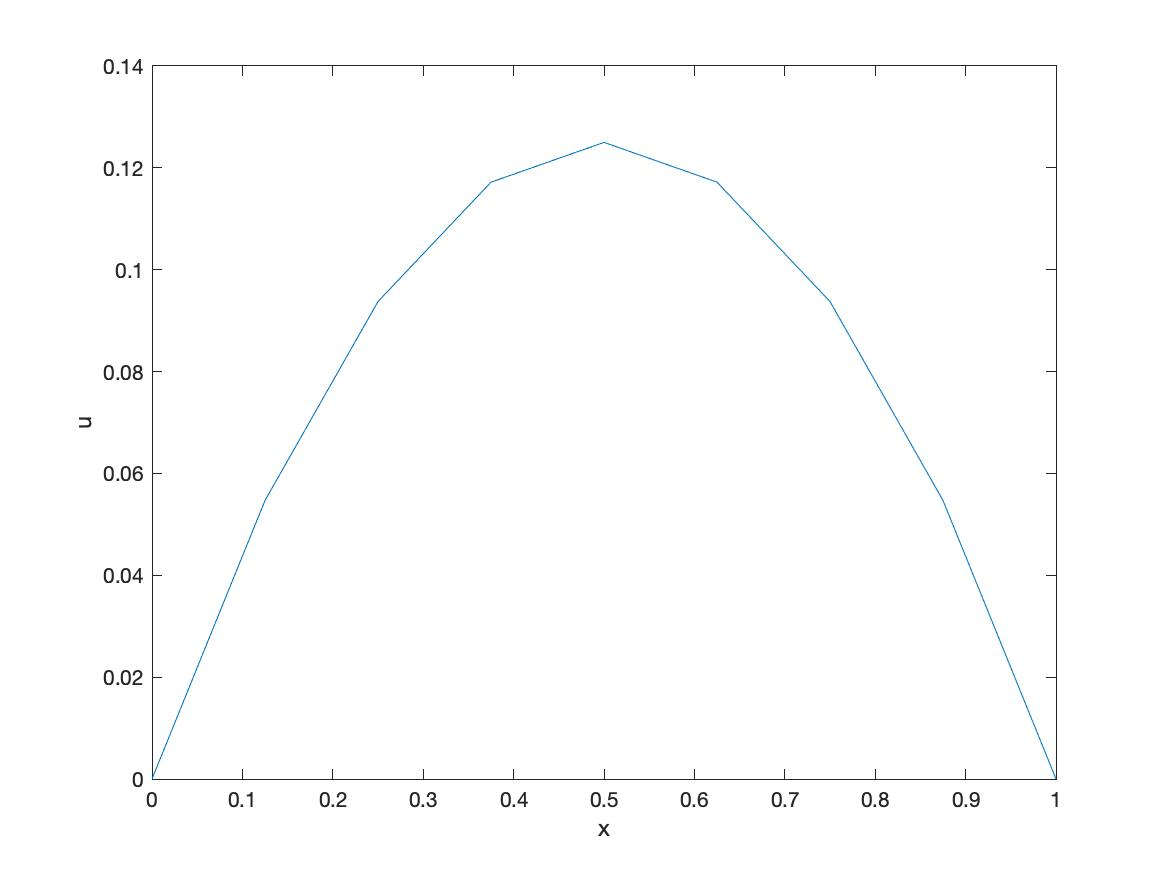
\includegraphics[width=0.6\textwidth]{solution.jpg} %Change to appropriate file name
\end{center}
\item[3(c)] 
Enter your your plot for $N=10$ below:
\begin{center}
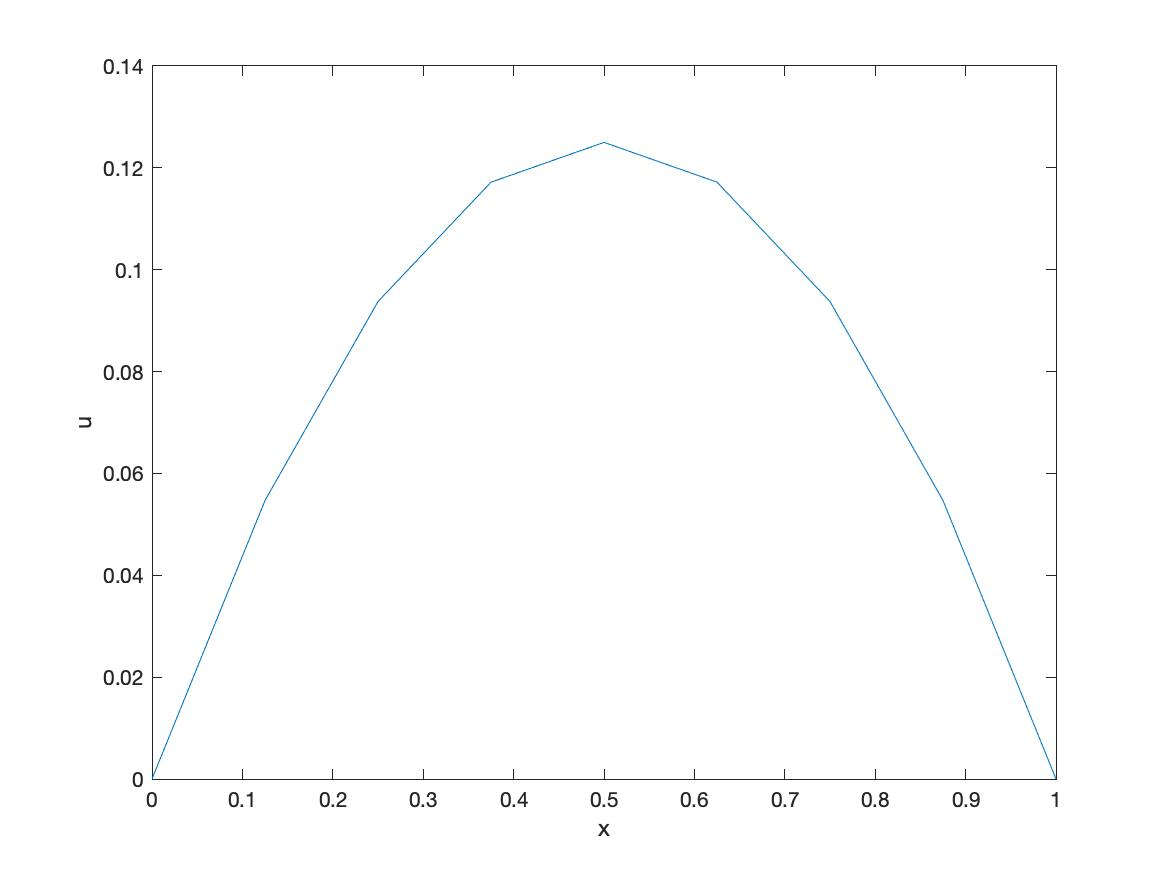
\includegraphics[width=0.6\textwidth]{solution.jpg} %Change to appropriate file name
\end{center}
Enter your your plot for $N=100$ below:
\begin{center}
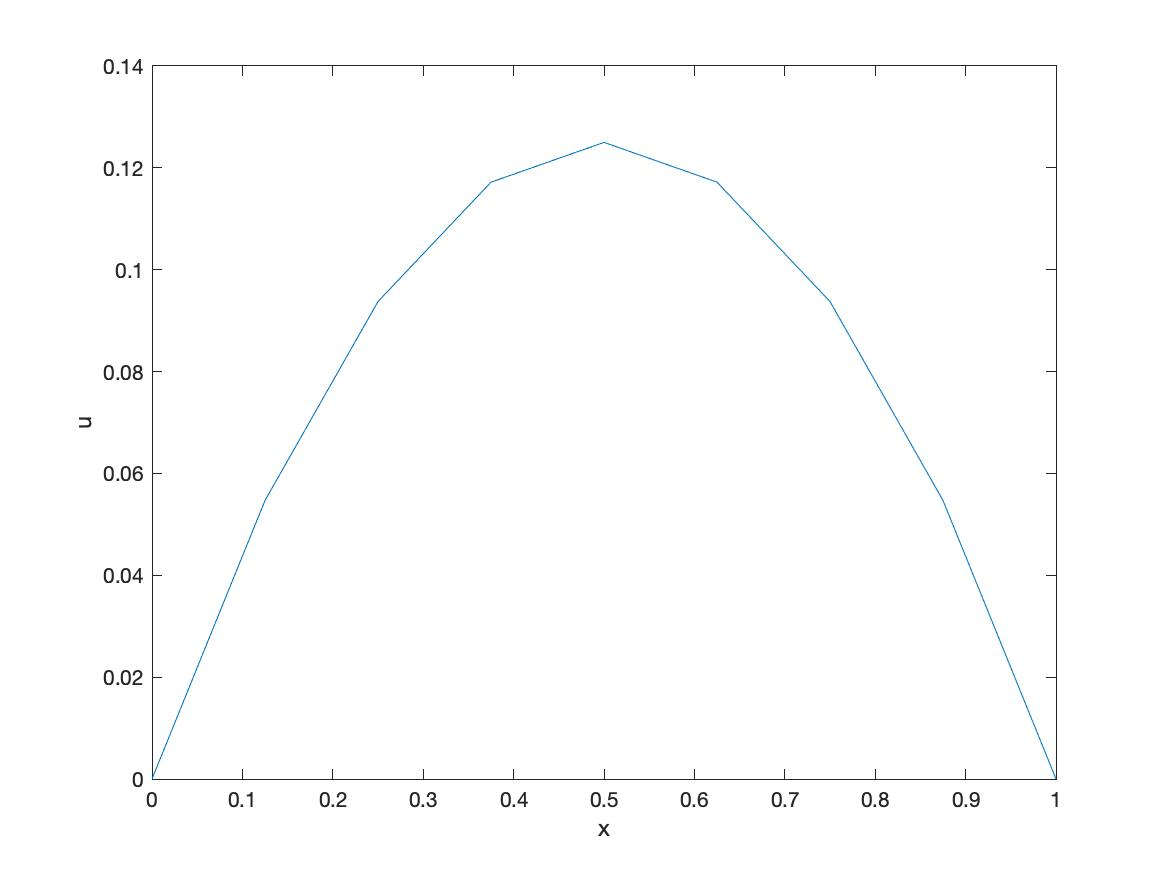
\includegraphics[width=0.6\textwidth]{solution.jpg} %Change to appropriate file name
\end{center}
\end{enumerate}
\end{document}
